% JuliaCon proceedings template
\documentclass{juliacon}
\setcounter{page}{1}
\input{racket-lang.tex}

\begin{document}

% **************GENERATED FILE, DO NOT EDIT**************

\title{Pattern-Based Syntax Analysis for Julia}

\author[1]{Iulia Maria Dumitru}
\affil[1]{University Politehnica of Bucharest}

\keywords{Julia, Racket, pattern matching, static analysis}

\hypersetup{
pdftitle = {Pattern-Based Syntax Analysis for Julia},
pdfsubject = {JuliaCon 2025 Proceedings},
pdfauthor = {Iulia Maria Dumitru},
pdfkeywords = {Julia, Racket, pattern matching, static analysis},
}



\maketitle

\begin{abstract}

In this thesis we present the implementation of a system for matching
syntax and writing static analysis rules in Julia. We begin by
describing Julia's metaprogramming capabilities and comparing them to
syntax manipulation libraries from the Racket ecosystem. We explain
the rationale for porting part of Racket's functionality to
Julia. After understanding the main principles behind the inspiration
libraries, we present our Julia implementation. The defined concepts
and algorithms are illustrated with instructive examples and the
system's flexibility is showcased in a real-world scenario. Finally,
we outline potential extensions and improvements for our
implementation.

\end{abstract}

\section{Introduction}
\label{sec:org3029f3b}

The ability to reason about \emph{code as data} is essential for writing
static analysis tools and is the quintessence of
metaprogramming. Compilers, interpreters, linters — they all
manipulate program inputs, whether it's for generating other programs,
evaluating expressions or signaling errors.

Languages that facilitate access to their own representation are
generally highly extendable and introspectable. Lisp is the canonical
example of a \emph{homoiconic} language, with S-expressions having been
invented specifically for unifying the representation of Lisp code and
data \cite{lisp_paper}. Lisp dialects rely on metaprogramming
(macros) to analyse, generate and transform programs dynamically.

Julia takes inspiration from Lisp in its ``willingness to represent
itself'' \cite{skarpinski_julia_willingness}. Like Lisp, it has a
powerful macro system that enables manipulating programs at the
syntactic level \cite{julia_metaprogramming}. But unlike Lisp, Julia
is a young language \cite{julia_creation} and has much to learn from
its older relatives in order to fully take advantage of its own
features.

\subsection{Syntax Manipulation in Julia}
\label{sec:org581a919}

Julia programs are represented as sequences of expressions — objects
of type \href{https://docs.julialang.org/en/v1/base/base/\#Core.Expr}{\texttt{Expr}}. Expressions have a head and a list of arguments, which
are themselves expressions\footnote{\href{https://docs.julialang.org/en/v1/manual/metaprogramming/\#Symbols}{Symbols} and atoms (\href{https://docs.julialang.org/en/v1/manual/metaprogramming/\#man-quote-node}{\texttt{QuoteNode}s}) are also representations of
Julia code. For conciseness, we refer to these as expressions as well.}. The Julia parser —
JuliaSyntax.jl\footnote{JuliaSyntax has been the default Julia parser since \href{https://github.com/JuliaLang/julia/releases/tag/v1.10.0}{Julia 1.10}
(2023). Before JuliaSyntax, the default parser was implemented in
\href{https://github.com/JuliaLang/julia/blob/master/src/julia-parser.scm}{femtolisp}.} — parses text and transforms it into syntax
trees. These can be directly \texttt{Expr}s or other tree representations
such as \texttt{SyntaxNode}s. The parser does not directly produce syntax
trees, allowing its output to be post-processed into any custom tree
data structure \cite{parse_stream}.

\texttt{SyntaxNode} data structures are richer than \texttt{Expr}s. They provide
detailed code provenance information and remain more faithful to the
code's textual representation \cite{syntax_nodes}. Code analysis
tools such as JET.jl \cite{jet} or Cthulhu.jl \cite{cthulhu} use and
extend \texttt{SyntaxNode}s for more flexibility and expressivity.

There are already a few syntax manipulation packages in the Julia
ecosystem. Some are widely used, including MacroTools.jl
\cite{macro_tools} and MLStyle.jl \cite{mlstyle}. However, they
don't fully exploit Julia's representational flexibility. Inspiration
can be drawn from research-oriented Lisp dialects, which explore
syntax matching and templating more extensively.

\subsection{Syntax Manipulation in Racket}
\label{sec:orgc44ac28}

Racket stands out among Lisps for being ``a programming language for
creating new programming languages'' \cite{racket_manifesto}. It
provides a powerful mechanism for parsing syntax and creating new
syntactic forms within Racket itself through the \texttt{syntax/parse}
library \cite{syntax_parse}.

The main focus of \texttt{syntax/parse} is writing robust macros that
automatically generate specific error messages for invalid
input. Macros are syntactic specifications defined with \emph{syntax
patterns} and \emph{syntax templates}. Patterns match pieces of syntax,
which get transformed into other pieces of syntax at compile time. The
transformation consists of filling in templates with \emph{pattern
variables} bound during pattern matching. Patterns can reference
\emph{syntax classes} for constraining pattern variables. Syntax classes
can be seen as abstractions over patterns that encapsulate syntactic
categories \cite{syntax_class}.

This framework forms the basis for Resyntax \cite{resyntax}, a Racket
refactoring library that allows writing and using suites of rules for
analysing and rewriting code. It provides a command line tool with two
commands: \texttt{resyntax analyze} and \texttt{resyntax fix}. The former analyses
files and prints suggestions specified in the refactoring rules
driving the analysis. The latter applies the suggestions directly to
the analysed code and prints a summary of the refactoring.

\subsection{Bringing Racket's Philosophy to Julia}
\label{sec:org2397f8a}

There is no technical limitation stopping Julia from attaining the
same level of expressivity as Racket when it comes to syntax
specification and analysis. Julia's code representation can be
reflected upon and restructured. Julia's macro system can be enriched
with pattern-matching macros. And static analysis tools for Julia can
build upon these macros to create versatile and reliable frameworks
for enforcing code standards.

This paper presents Argus.jl, a Julia package for pattern-based static
analysis inspired by Racket's \texttt{syntax/parse} and Resyntax libraries.

\section{Understanding the Inspiration Model}
\label{sec:orga631655}

\subsection{Background and Motivation Behind \texttt{syntax/parse}}
\label{sec:org0a134f1}

Before \texttt{syntax/parse}, the state of the art for writing macros was
Macro-by-Example (MBE) \cite{mbe}. MBE was developed as a Lisp
specification language allowing a declarative specification of
macros\footnote{The concept gained popularity and started being implemented in
other languages, most famously in \href{https://doc.rust-lang.org/reference/macros-by-example.html}{Rust}.}. In their 1986 paper introducing the notation,
Kohlbecker and Wand offer an example with the familiar \texttt{let}
expression implemented as a lambda function application\footnote{All examples in this section are either adaptations or direct
reproductions from the cited sources.}:

\begin{lstlisting}[language=racket]
(let ((i e) ...) b ...)
  ==> ((lambda (i ...) b ...) e ...)
\end{lstlisting}

This specification states that a \texttt{let} expression expects zero or more
\emph{binding pairs} (\texttt{(i e) ...}) and zero or more body expressions \\ (\texttt{b ...}). It is semantically equivalent to a lambda function with zero or
more formal parameters (\texttt{i ...}) — corresponding to the bound
variables in the \texttt{let} form — and a body containing zero or more
expressions (\texttt{b ...}), applied to zero or more actual parameters (\texttt{e ...}). Defining \texttt{let} as a macro without the MBE notation requires
carefully destructuring and reassembling input code:

\begin{lstlisting}[language=racket]
(defmacro let (decls . body)
  `((lambda ,(map car decls) . ,body)
    . ,(map cadr decls)))
\end{lstlisting}

It is difficult to distinguish the macro's input and output shapes by
reading this definition. Validating the input in order to generate
useful error messages would further complicate the definition, making
it almost incomprehensible\footnote{The definition is already incomprehensible for the reader who
is not familiar with Lisp.}.

With MBE, a \texttt{let} definition can resemble the specification much more
closely:

\begin{lstlisting}[language=racket]
(declare-syntax let
  [(let ((i e) ...) b ...)
   ((lambda (i ...) b ...) e ...)])
\end{lstlisting}

The syntactic shape of the input is validated automatically through
pattern matching. This eliminates the need to write explicit code for
structural validation. The variables bound when matching the \emph{pattern}
— \texttt{(let ((i e) ...) b ...)} — are used to fill in the \emph{template} —
\texttt{((lambda (i ...) b ...) e ...)} — and generate the resulting
code. Additional checks are still necessary to ensure the correct use
of a \texttt{let} expression. For example, there should be a condition
verifying that all bound identifiers are unique. MBE lacks a
straightforward representation for such conditions.

In the 2012 article ``Fortifying Macros'' \cite{fortifying_macros},
Ryan Culpepper explains in more detail the limitations of the MBE
notation, presenting a strong case for creating a new system. A \texttt{let}
macro that fully validates its input can be written clearly and
concisely in this new framework:

\begin{lstlisting}[language=racket]
(define-syntax (let stx)
  (syntax-parse stx
    [(let ([var:identifier rhs:expr] ...) body:expr)
     #:fail-when (check-duplicate #'(var ...))
                 "duplicate variable name"
     #'((lambda (var ...) body) rhs ...)]))
\end{lstlisting}

First, \texttt{syntax-parse} verifies that the input syntax matches the
pattern in the first clause of its body — \texttt{(let ([var:identifier
rhs:expr] ...) body:expr)}. Then, it asserts that there are no
duplicates in the identifier list bound to \texttt{var}. If there are, the
parsing fails with the message ``duplicate variable name''. Finally,
if all checks succeeded the input is transformed into the new syntax
specified by the template in the last clause — \texttt{\#’((lambda (var ...)
body) rhs ...)}.

Given correct input, the above \texttt{let} implementation expands to the
corresponding lambda application at compile time and evaluates the
application at run time. Given incorrect input, a specific error is
thrown at compile time.

\vspace{1em}

\noindent
\texttt{(let ([a 1] [b 2]) (+ a b))}

\vspace{0.05cm}
\noindent\hspace{0.3cm}\textit{compile-time expansion}: \texttt{((lambda (a b) (+ a b)) 1 2)}

\noindent\hspace{0.3cm}\textit{run-time result}: \texttt{3}

\vspace{0.25cm}

\noindent
\texttt{(let (["a" 1]) (add1 a))}

\noindent\hspace{0.3cm}\textit{compile-time error}: \texttt{expected identifier}

\vspace{0.25cm}

\noindent
\texttt{(let ([a 1] [a 2]) (+ a a))}

\noindent\hspace{0.3cm}\textit{compile-time error}: \texttt{duplicate variable name}

\vspace{1em}

Misuses that are not explicitly covered by the \texttt{syntax-parse}
definition generate a generic error message.

\vspace{1em}

\noindent
\texttt{(let (x 5) (add1 x))}

\noindent\hspace{0.3cm}\textit{compile-time error}: \texttt{bad syntax}

\subsection{Building Blocks}
\label{sec:org3aeafde}

The layout of a macro definition in \texttt{syntax/parse} consists of
\emph{patterns} and \emph{templates}. Patterns match input code, binding
\emph{pattern variables} in the process. Pattern variables can be annotated
by \emph{syntax classes} in order to refine matching and error-reporting.

The definition of \texttt{let} in the previous sub-section contains three
pattern variables: \texttt{var}, \texttt{rhs} and \texttt{body}. Because \texttt{var} and \texttt{rhs}
are surrounded by an \emph{ellipsis}, they have an \emph{ellipsis depth}
of 1. \texttt{body} does not have any ellipses around it and has ellipsis
depth 0. Ellipses can be nested to any depth. A variable appearing in
the pattern at ellipsis depth \emph{d} must appear in the template at the
same depth.

All pattern variables in the \texttt{let} pattern have explicit syntax class
annotations — \texttt{expr} for \texttt{rhs} and \texttt{body} and \texttt{identifier} for
\texttt{var}. A syntax class groups together ``syntactically similar'' forms
and associates them with a corresponding class of errors.

Error reporting for \texttt{let} can be further improved by defining a syntax
class corresponding to binding pairs and rewriting \texttt{let}:

\begin{lstlisting}[language=racket]
(define-syntax-class binding
  #:description "binding pair"
  (pattern [var:identifier rhs:expr]))

(define-syntax (let stx)
  (syntax-parse stx
    [(let (b:binding ...) body:expr)
     #:fail-when (check-duplicate #'(b.var ...))
                 "duplicate variable name"
     #'((lambda (b.var ...) body) b.rhs ...)]))
\end{lstlisting}

If \texttt{b} binds to anything other than a binding pair, a specific error
message is shown rather than the generic ``bad syntax'':

\vspace{1em}

\texttt{(let (x 5) (add1 x))}

\hspace{0.3cm}\textit{compile-time error}: \texttt{expected binding pair}

\subsection{Resyntax}
\label{sec:org37726eb}

Even though \texttt{syntax/parse} is centered around writing macros, it can
also form the basis for tools that identify problematic patterns in
code. The Resyntax library \cite{resyntax} leverages its capabilities
for matching patterns and rewriting code to implement such a tool.

Resyntax allows the definition of \emph{refactoring rules}, which are
``macro-like functions defined in terms of \texttt{syntax-parse} that specify
how to search for and refactor different coding patterns''. A rule
matches patterns in source code and makes a refactoring suggestion
with an associated description.

The following rule searches for unnecessarily nested \texttt{or} expressions:

\begin{lstlisting}[language=racket]
(define-refactoring-rule nested-or-to-flat-or
  #:description "This nested `or` expression can be flattened."
  #:literals (or)
  (or a (or b c))
  (or a b c))
\end{lstlisting}

The first line in the body contains the rule's description. The second
line provides a list of identifiers that should be treated as literals
instead of pattern variables. The third and fourth lines define the
pattern to be searched for and the template for generating the
refactored \texttt{or} expression, respectively.

Refactoring rules can be grouped in \emph{refactoring suites}. Resyntax
comes with a default refactoring suite. The user is free to use the
default or define custom rules and suites to fit their needs.

\section{Adapting the Model to Julia}
\label{sec:org7db2573}

\href{https://github.com/iuliadmtru/Argus.jl}{Argus.jl} was created to explore Julia's ability to offer highly
expressive syntax manipulation tools similar to Racket's. It extends
the Julia parser with a custom tree data structure for representing
patterns. Its pattern matching capabilities exceed the scope of
existing pattern matching Julia packages such as MacroTools.jl
\cite{macro_tools}. Like Resyntax, Argus builds upon the syntax
matching framework to create a powerful mechanism for writing static
analysis rules.

The scope of Argus is currently limited to matching syntax and writing
rules that search for patterns in code. However, it can be easily
extended to include templating facilities for code refactoring.

\subsection{Overview of Julia's Syntax}
\label{sec:org1f20944}

The effectiveness of a metaprogramming tool is strongly influenced by
the extent of the information it can access. Julia's surface syntax
\texttt{Expr}s are annotated with \texttt{LineNumberNodes} to provide source
location information \cite{julia_asts}. This information is limited
to line number and file name. The code structure can be investigated
by looking at the head and arguments of its \texttt{Expr} representation.

The following examples illustrate the structure of \texttt{Expr}s. The
expressions are evaluated in the Julia REPL \cite{julia_repl}.

\begin{lstlisting}[language=Julia]
julia> toplevel_expr = Meta.parseall("""
                                     x = :x
                                     println(x, 2)
                                     """);

julia> toplevel_expr.head
:toplevel

julia> toplevel_expr.args
4-element Vector{Any}:
 :(#= none:1 =#)
 :(x = :x)
 :(#= none:2 =#)
 :(println(x, 2))
\end{lstlisting}

\texttt{Meta.parseall} parses a series of toplevel expressions into an \texttt{Expr}
with a \texttt{:toplevel} head\footnote{The equivalent for single expressions is \texttt{Meta.parse}.}.

\texttt{LineNumberNodes} are printed inside block comments (\texttt{\#=...=\#}). They
indicate the file in which the annotated expression was executed
(\texttt{none} indicates REPL execution) and the line at which it appears in
the source text.

\texttt{x = :x} is an assignment expression with two children — the
identifier \texttt{x} and the \texttt{Symbol} \texttt{:x}. \texttt{println(x, 2)} is a function
call with three children — the function name, \texttt{println}, and two
function arguments, \texttt{x} and \texttt{2}.

\begin{lstlisting}[language=Julia]
julia> toplevel_expr.args[2].head
:(=)

julia> toplevel_expr.args[2].args
2-element Vector{Any}:
 :x
 :(:x)

julia> toplevel_expr.args[4].head
:call

julia> toplevel_expr.args[4].args
3-element Vector{Any}:
  :println
  :x
2
\end{lstlisting}

Extracting information from \texttt{LineNumberNode}s can be unintuitive and
limiting. A \texttt{LineNumberNode} is not directly attached to the
expression it annotates. Instead, it appears as a sibling node located
immediately above the corresponding expression. Moreover, it has no
knowledge of the expression's textual representation.

\texttt{Expr}s can also cause confusion. In an \texttt{Expr} an identifier is
represented as a \texttt{Symbol}. A \texttt{Symbol} is a \texttt{QuoteNode}. Literals are
anything other than \texttt{Expr}, \texttt{Symbol} and \texttt{QuoteNode}.

\begin{lstlisting}[language=Julia]
julia> typeof(:( x = 2 ))
Expr

julia> typeof(:( x ))
Symbol

julia> typeof(:( :x ))
QuoteNode

julia> typeof(:( "abc" ))
String
\end{lstlisting}

JuliaSyntax's \texttt{SyntaxNode}s facilitate access to code-related
information. They retain all syntactic trivia such as whitespace and
comments \cite{juliasyntax}, making it possible to determine an
expression's byte span. The type of a \texttt{SyntaxNode} is denoted as a
``syntax kind'' \cite{js_kinds}, allowing the efficient definition of
predicates such as \texttt{is\_identifier} and \texttt{is\_operator}.

\begin{lstlisting}[language=Julia]
julia> using JuliaSyntax: JuliaSyntax, SyntaxNode, parsestmt, parseall, kind, source_location, byte_range, is_identifier, is_literal

julia> toplevel_node =
           parseall(SyntaxNode, """
                                x = :x
                                println(x, 2)
                                """)
SyntaxNode:
[toplevel]
  [=]
    x                                :: Identifier
    [quote-:]
      x                              :: Identifier
  [call]
    println                          :: Identifier
    x                                :: Identifier
    2                                :: Integer


julia> kind(toplevel_node)
K"toplevel"

julia> toplevel_node.children
2-element Vector{SyntaxNode}:
 (= x (quote-: x))
 (call println x 2)

julia> kind(toplevel_node.children[1])
K"="

julia> kind(toplevel_node.children[2])
K"call"

julia> source_location(toplevel_node.children[2])
(2, 1)

julia> byte_range(toplevel_node.children[2])
8:20

julia> is_identifier(parsestmt(SyntaxNode, "x"))
true

julia> is_identifier(parsestmt(SyntaxNode, ":x"))
false

julia> is_literal(parsestmt(SyntaxNode, "2"))
true
\end{lstlisting}

The parsing functions from JuliaSyntax can produce both \texttt{Expr}s and
\texttt{SyntaxNode}s, among other tree types \cite{juliasyntax}. The result
type is specified by the first argument.

A \texttt{SyntaxNode} is implemented as a concrete subtype of the generic
type \texttt{TreeNode}. \texttt{TreeNode}s can be extended to create custom
syntactic representations.

\begin{lstlisting}[language = Julia]
mutable struct TreeNode{NodeData}
    parent::Union{Nothing, TreeNode{NodeData}}
    children::Union{Nothing,
                    Vector{TreeNode{NodeData}}}
    data::Union{Nothing, NodeData}

    ...
end

const SyntaxNode = TreeNode{SyntaxData}
\end{lstlisting}

\texttt{SyntaxData} is a data structure that holds information such as source
location and syntax kind. Its implementation is not important for our
purposes.

Because of the advantages of \texttt{SyntaxNode} over \texttt{Expr}, Argus uses
\texttt{SyntaxNode}s to represent Julia code.

\subsection{Implementing Argus.jl}
\label{sec:orgaa377d4}

Argus can be split in two distinct components:

\begin{itemize}
\item a syntax matching mechanism;
\item a framework for writing rules.
\end{itemize}

The former provides the necessary building blocks for defining an
\emph{embedded domain-specific language} \cite{dsl} for syntax
matching. It implements the fundamental concepts behind
\texttt{syntax/parse}, borrowing syntactic representation for some of the
constructs.

The latter extends this syntax matching language with implementations
for \emph{rules} and \emph{rule groups}. These are inspired by Resyntax's
\emph{refactoring rules} and \emph{refactoring suites} but are currently limited
to searching for patterns in code.

\subsubsection{Matching Syntax}
\label{sec:orgc7e5599}

A syntax matching engine needs to define two essential concepts:
\emph{patterns} and the \emph{criteria for compatibility} between a pattern and
a syntax object.

Argus defines patterns in terms of regular abstract syntax tree nodes
(hereafter referred to as simply \emph{syntax nodes}) and special nodes
denoting \emph{pattern forms} \cite{pattern_forms}. Pattern nodes are
implemented by extending the \texttt{TreeNode} type described in section
\ref{sec:org1f20944} with a \texttt{SyntaxPatternNode} type. A
\texttt{SyntaxPatternNode} can either carry regular \texttt{SyntaxNode} data or
pattern form-specific data.

\begin{lstlisting}[language=Julia]
const SyntaxPatternNode = Juliasyntax.TreeNode{
    Union{JuliaSyntax.SyntaxData,
          AbstractPatternFormSyntaxData}
}
\end{lstlisting}

A \texttt{Pattern} is a light wrapper around a \texttt{SyntaxPatternNode}.

\begin{lstlisting}[language=Julia]
struct Pattern
    src::SyntaxPatternNode
end
\end{lstlisting}

\texttt{Pattern}s and \texttt{SyntaxPatternNode}s only differ in their level of
abstraction. A \texttt{Pattern} represents the higher level notion of a
\emph{syntax pattern}. A \texttt{SyntaxPatternNode} is the implementation of a
syntax pattern — its representation as an \emph{abstract syntax
tree}. Since we are discussing implementation details, we will be
using the terms \emph{pattern} and \emph{pattern node} interchangeably.

\phantomsection\label{orga8b3c0d}\vspace{0.5cm}
\textbf{Pattern Forms}\vspace{0.2cm}

Argus implements five pattern forms. When defining patterns, a pattern
form can appear explicitly as \texttt{\textasciitilde{}<form-name>(<form-args>...)} or
implicitly in its syntactic-sugar notation.

\vspace{0.2cm}
\phantomsection\label{org831c838}\vspace{0.2cm}
\underline{\texttt{\textasciitilde{}var}}

\begin{lstlisting}[language=Julia]
struct VarSyntaxData <: AbstractPatternFormSyntaxData
    var_name::Symbol
    syntax_class_name::Symbol
end
\end{lstlisting}

A \texttt{\textasciitilde{}var} form associates a pattern variable with a syntax class. The
following representations of \texttt{\textasciitilde{}var} are equivalent:

\begin{lstlisting}[language=Julia]
julia> @pattern ~var(:x, :expr)
Pattern:
x:::expr                             :: ~var

julia> @pattern {x:::expr}
Pattern:
x:::expr                             :: ~var

julia> @pattern {x}
Pattern:
x:::expr                             :: ~var
\end{lstlisting}

Syntax classes referenced by a \texttt{\textasciitilde{}var} pattern need to be registered in
a \emph{syntax class registry} before match time\footnote{The notion of a syntax class registry is general and its
implementation is not important. For the curious reader, Argus
represents it as a dictionary mapping syntax class names to
definitions.}.

\vspace{0.2cm}
\phantomsection\label{org3caafc9}\vspace{0.2cm}
\underline{\texttt{\textasciitilde{}fail}}

\begin{lstlisting}[language=Julia]
struct FailSyntaxData <: AbstractPatternFormSyntaxData
    condition::Function
    message::String

    FailSyntaxData(cond, msg::String) =
        new(fail_condition(cond), msg)
end
\end{lstlisting}

A \texttt{\textasciitilde{}fail} form causes a pattern match to fail if a given condition is
satisfied, providing a relevant failure message. The condition can
reference previously-bound pattern variables.

\begin{lstlisting}[language=Julia]
julia> fail = @pattern ~fail([],
                             true,
                             "always fails")
Pattern:
[~fail]
  true                               :: Bool
  "always fails"                     :: String

julia> syntax_match(fail,
                    parsestmt(SyntaxNode,
                              "dummy"))
MatchFail("always fails")

julia> fail_if_even = @pattern ~and(
           {n},
           ~fail([:n],
                 iseven(n.value),
                 "expected odd")
       )
Pattern:
[~and]
  n:::expr                           :: ~var
  [~fail]
    [call]
      iseven                         :: Identifier
      [.]
        n                            :: Identifier
        value                        :: Identifier
    "expected odd"                   :: String

julia> syntax_match(fail_if_even,
                    parsestmt(SyntaxNode,
                              "2"))
MatchFail("expected odd")

julia> syntax_match(fail_if_even,
                    parsestmt(SyntaxNode,
                              "3"))
BindingSet with 1 entry:
  :n => Binding:
          Name: :n
          Bound source: 3 @ 1:1
          Ellipsis depth: 0
          Sub-bindings:
            BindingSet with 0 entries
\end{lstlisting}

The \texttt{FailSyntaxData} constructor expects a condition expression and a
failure message. The condition expression is processed into an
anonymous function that takes as argument a set of pattern variable
bindings. During matching, when the function is called, the pattern
variables are defined in its evaluation context. The condition
expression is then evaluated in the same context. All pattern
variables referenced in the fail condition should have associated
bindings at match time.

\texttt{\textasciitilde{}fail} can be written as a \texttt{@fail} macro inside a pattern. Pattern
fail conditions in the \texttt{@fail} form require the pattern to be written
as a sequence of expressions using a \texttt{begin ... end} block
\cite{compound_exprs}. The expressions above the first fail condition
are interpreted as toplevel expressions. Fail conditions and toplevel
expressions are combined into an \texttt{\textasciitilde{}and} pattern. They cannot be
interspersed.

\begin{lstlisting}[language=Julia]
julia> @pattern begin
           expr1
           expr2
           @fail [] condition "message"
       end
Pattern:
[~and]
  [toplevel]
    expr1                            :: Identifier
    expr2                            :: Identifier
  [~fail]
    condition                        :: Identifier
    "message"                        :: String

julia> @pattern begin
           expr1
           @fail [] condition "message"
           expr2
       end
ERROR: LoadError: SyntaxError: invalid `@pattern` syntax
Pattern expressions and fail conditions cannot be interspersed.
...
\end{lstlisting}

The \texttt{@fail} macro has no meaning outside of pattern definitions.

\begin{lstlisting}[language=Julia]
julia> @fail [] condition "message"
ERROR: LoadError: UndefVarError: `@fail` not defined in `Main`
...
\end{lstlisting}

\vspace{0.9cm}
\phantomsection\label{orgc8372d0}\vspace{0.2cm}
\underline{\texttt{\textasciitilde{}or}}

\begin{lstlisting}[language=Julia]
struct OrSyntaxData <: AbstractPatternFormSyntaxData end
\end{lstlisting}

\texttt{\textasciitilde{}or} combines one or more patterns with short-circuiting logical \texttt{or}
semantics. \texttt{\textasciitilde{}or} forms only have explicit notation.

\begin{lstlisting}[language=Julia]
julia> equals_x = @pattern ~or(
           x == {first},
           {second} == x
       )
Pattern:
[~or]
  [call-i]
    x                                :: Identifier
    ==                               :: Identifier
    first:::expr                     :: ~var
  [call-i]
    second:::expr                    :: ~var
    ==                               :: Identifier
    x                                :: Identifier

julia> syntax_match(equals_x,
                    parsestmt(SyntaxNode,
                              "x == 2"))
BindingSet with 1 entry:
  :first => Binding:
              Name: :first
              Bound source: 2 @ 1:6
              Ellipsis depth: 0
              Sub-bindings:
                BindingSet with 0 entries

julia> syntax_match(equals_x,
                    parsestmt(SyntaxNode,
                              "2 == x"))
BindingSet with 1 entry:
  :second => Binding:
               Name: :second
               Bound source: 2 @ 1:1
               Ellipsis depth: 0
               Sub-bindings:
                 BindingSet with 0 entries
\end{lstlisting}

\vspace{0.2cm}
\phantomsection\label{orgfe488bd}\vspace{0.2cm}
\underline{\texttt{\textasciitilde{}and}}

\begin{lstlisting}[language=Julia]
struct AndSyntaxData <: AbstractPatternFormSyntaxDataend
\end{lstlisting}

\texttt{\textasciitilde{}and} combines one or more patterns with short-circuiting logical
\texttt{and} semantics. Like \texttt{\textasciitilde{}or}, \texttt{\textasciitilde{}and} can only be written explicitly.

\begin{lstlisting}[language=Julia]
julia> conflicting_and = @pattern ~and({a} + 2,
                                       {a} + 3)
Pattern:
[~and]
  [call-i]
    a:::expr                         :: ~var
    +                                :: Identifier
    2                                :: Integer
  [call-i]
    a:::expr                         :: ~var
    +                                :: Identifier
    3                                :: Integer

julia> syntax_match(conflicting_and, parsestmt(SyntaxNode, "a + 2"))
MatchFail("no match")
\end{lstlisting}

\vspace{0.2cm}
\phantomsection\label{orge098f9d}\vspace{0.2cm}
\underline{\texttt{\textasciitilde{}rep}}

\begin{lstlisting}[language=Julia]
struct RepSyntaxData <: AbstractPatternFormSyntaxData
    rep_vars::Vector{RepVar}
end
\end{lstlisting}

\texttt{\textasciitilde{}rep} denotes a pattern wrapped in one level of \emph{ellipses},
indicating it may repeat zero or more times. Nested \texttt{\textasciitilde{}rep} forms are
allowed within the enclosed pattern.

\begin{lstlisting}[language=Julia]
julia> match_all = @pattern ~rep({ex})
Pattern:
[~rep]
  ex:::expr                          :: ~var

julia> syntax_match(match_all,
                    parseall(SyntaxNode, """
                                         x = 2
                                         x + 1
                                         """))
BindingSet with 1 entry:
  :ex => Binding:
           Name: :ex
           Bound sources: [(= x 2) @ 1:1,
                           (call-i x + 1) @ 2:1]
           Ellipsis depth: 1
           Sub-bindings:
             [
              BindingSet with 0 entries,
              BindingSet with 0 entries
             ]
\end{lstlisting}

A \texttt{\textasciitilde{}rep} form may be represented implicitly using ellipses. The above
\texttt{match\_all} pattern can be rewritten as \texttt{@pattern \{ex\}...}.

The sugared \texttt{\textasciitilde{}rep} notation hijacks Julia's built-in \href{https://docs.julialang.org/en/v1/base/base/\#...}{splat
operator}. It is possible to refer to the splat operator instead of
\texttt{\textasciitilde{}rep} in a pattern by escaping the pattern expression.

\begin{lstlisting}[language=julia]
julia> @pattern v...
Pattern:
[~rep]
  v                                  :: Identifier
julia> @pattern @esc(v...)
Pattern:
[...]
  v                                  :: Identifier
\end{lstlisting}

\texttt{@esc} escapes the entire encapsulated expression by default, but
supports specifying a custom escape level.

\begin{lstlisting}[language=julia]
julia> @pattern @esc([{elems}...]...)
Pattern:
[...]
  [vect]
    [...]
      [braces]
        elems                        :: Identifier

julia> @pattern @esc([{elems}...]..., 1)
Pattern:
[...]
  [vect]
    [~rep]
      elems:::expr                   :: ~var

julia> @pattern @esc([{elems}...]..., 3)
Pattern:
[...]
  [vect]
    [...]
      elems:::expr                   :: ~var
\end{lstlisting}

\vspace{0.2cm}
\phantomsection\label{orge75d301}\vspace{0.2cm}
\textbf{Syntax Classes}\vspace{0.2cm}

\texttt{\textasciitilde{}var} forms reference syntax classes in patterns. Matching a pattern
that references an unregistered syntax class causes a match time
error.

\begin{lstlisting}[language=julia]
julia> syntax_match((@pattern {x:::unregistered}),
                    parsestmt(SyntaxNode, "dummy"))
ERROR: SyntaxClassRegistryKeyError: unregistered
syntax class :unregistered
...
\end{lstlisting}

Syntax classes can be defined using the \texttt{@syntax\_class} macro. They
follow the behaviour described in section \ref{sec:org3aeafde} for
\texttt{syntax/parse}. A syntax class contains a description and a sequence
of one or more patterns.

\begin{lstlisting}[language=julia]
julia> vec = @syntax_class "vector" begin
           @pattern [{_}...]
       end
SyntaxClass: vector
  Pattern alternative #1:
    [vect]
      [~rep]
        _:::expr                     :: ~var

julia> syntax_match(vec,
                    parsestmt(SyntaxNode,
                              "[1, [2]]"))
BindingSet with 0 entries
\end{lstlisting}

In order to use them in patterns, syntax classes need to be
registered.

\begin{lstlisting}[language=julia]
julia> register_syntax_class!(:vec, vec);

julia> vec_of_vecs = @pattern [{v:::vec}...];

julia> syntax_match(vec_of_vecs,
                    parsestmt(SyntaxNode,
                              "[[1, 2], [[3]]]"))
BindingSet with 1 entry:
  :v => Binding:
          Name: :v
          Bound sources: [(vect 1 2) @ 1:2,
                          (vect (vect 3)) @ 1:10]
          Ellipsis depth: 1
          Sub-bindings:
            ...
\end{lstlisting}

Argus provides a set of pre-defined syntax classes, including
\texttt{vec}. The built-in implementations use \texttt{@define\_syntax\_class} to both
define and register syntax classes at the same time. The following is
Argus's implementation of the \texttt{fundef} syntax class:

\begin{lstlisting}[language=julia]
@define_syntax_class :fundef "function def" begin
    @pattern {call:::funcall} = {body}
    @pattern function ({call:::funcall})
        {body}...
    end
end
\end{lstlisting}

Writing multiple patterns in a \texttt{@syntax\_class} body is semantically
equivalent to combining the patterns in an \texttt{\textasciitilde{}or} form.

A bound pattern variable inherits all the pattern variables bound by
its constraining syntax class as sub-bindings, which can be accessed
as fields.

\begin{lstlisting}[language=julia]
@pattern begin
    {x:::assign}
    @fail x.rhs.value == 2 "rhs is two"
end
\end{lstlisting}

\phantomsection\label{org718abd6}\vspace{0.2cm}
\textbf{Comparing Patterns}\vspace{0.2cm}

The basic operation for matching syntax is the comparison of syntactic
objects. In the general case, Argus considers two syntax nodes to be
\emph{compatible} with each other if:

\begin{itemize}
\item they have the same head;
\item they contain the same value (or neither contains a value);
\item they are either both leafs, or both non-leafs and the children list
of one node is compatible with the children list of the other.
\end{itemize}

A \texttt{\textasciitilde{}var} node \emph{v} is compatible with a \texttt{SyntaxNode} \emph{s} if the syntax
class constraining the pattern variable referenced by \emph{v} is
compatible with \emph{s}. The pattern variable needs to be either unbound
or bound to a \texttt{SyntaxNode} compatible with \emph{s}. Matching \emph{v} with \emph{s}
binds its pattern variable to \emph{s}. A \texttt{\textasciitilde{}var} node inside a \texttt{\textasciitilde{}rep} node
is compatible with a \texttt{SyntaxNode} regardless of whether its pattern
variable is already bound. Pattern variable binding is handled by
\texttt{\textasciitilde{}rep}.

\texttt{\textasciitilde{}fail} nodes are not compared with other nodes. A \texttt{\textasciitilde{}fail} node \emph{f}
passes a comparison test if all the pattern variables referenced in
\emph{f}'s fail condition are bound and the fail condition is not
satisfied.

An \texttt{\textasciitilde{}or} node \emph{o} is compatible with a \texttt{SyntaxNode} \emph{s} if any of
\emph{o}'s branches is compatible with \emph{s}. During matching, \emph{o} records
all potentially succeeding paths encountered as \emph{recovery states}.

An \texttt{\textasciitilde{}and} node \emph{a} is compatible with a \texttt{SyntaxNode} \emph{s} if all \emph{a}'s
branches are compatible with \emph{s}. In case of incompatibility, the
matching tries to backtrack through available recovery states. Like
\emph{o}, \emph{a} records possible recovery states. It inherits and combines
the recovery states of its branches. The combined result can be
thought of as the cartesian product of the branches' recovery states.

A \texttt{\textasciitilde{}rep} node \emph{r} is compatible with a \texttt{SyntaxNode} \emph{s} if the node
enclosed in \emph{r} is compatible with \emph{s}. \emph{r} is compatible with a
sequence of \texttt{SyntaxNode}s \emph{ss} if \emph{ss} is empty or if the node
enclosed in \emph{r} is compatible with all the nodes in \emph{ss}. Matching \emph{r}
binds pattern variables to sequences of nodes. Like \emph{o} and \emph{a}, \emph{r}
tracks recovery states. During the matching of \emph{ss} with a \texttt{\textasciitilde{}rep} node
\emph{rc} contained in a complex pattern, \emph{rc} greedily consumes all the
nodes it can by default. It is possible to change the behaviour to a
non-greedy one.

\begin{lstlisting}[language=julia]
julia> ones = @pattern [
           1,
           ones1}...,
           1,
           {ones2}...
       ];

julia> syntax_match(ones, parsestmt(SyntaxNode, "[1, 1, 1, 1]"))
BindingSet with 2 entries:
  :ones2 => Binding:
              Name: :ones2
              Bound sources: []
              Ellipsis depth: 1
              Sub-bindings:
                []
  :ones1 => Binding:
              Name: :ones1
              Bound sources: [1 @ 1:5, 1 @ 1:8]
              Ellipsis depth: 1
              Sub-bindings:
                [
                 BindingSet with 0 entries,
                 BindingSet with 0 entries
                ]

julia> syntax_match(ones,
                    parsestmt(SyntaxNode,
                              "[1, 1, 1, 1]");
                    greedy=false)
BindingSet with 2 entries:
  :ones2 => Binding:
              Name: :ones2
              Bound sources: [1 @ 1:8, 1 @ 1:11]
              Ellipsis depth: 1
              Sub-bindings:
                [
                 BindingSet with 0 entries,
                 BindingSet with 0 entries
                ]
  :ones1 => Binding:
              Name: :ones1
              Bound sources: []
              Ellipsis depth: 1
              Sub-bindings: []
\end{lstlisting}

Only \texttt{\textasciitilde{}var} and \texttt{\textasciitilde{}rep} nodes can bind pattern variables.

\subsubsection{Writing Rules}
\label{sec:org73a41cd}

A rule is specified by its name, description and pattern.

\begin{lstlisting}[language=julia]
struct Rule
    name::String
    description::String
    pattern::Pattern
end
\end{lstlisting}

A rule match recursively traverses a given unit of source code and
collects the results of matching sub-expressions with the rule's
pattern. Bound pattern variables are returned in corresponding binding
sets \cite{argus_overview}.

\begin{lstlisting}[language=julia]
julia> assignments = @rule "assignments" begin
           description = """
           Searching for assignments.
           """
           pattern = @pattern {a:::assign}
       end
assignments: Searching for assignments.
Pattern:
a:::assign                           :: ~var

julia> src = """
       x = 2
       y = x + 1
       if y == x
           z = true
       end
       f() = 4
       """;

julia> match_result =
           rule_match(assignments,
                      parseall(SyntaxNode, src))
MatchResults with 3 matches and 0 failures:
Matches:
  BindingSet(:a => Binding(:a,
                           (= x 2) @ 1:1,
                           BindingSet(:rhs=>...,
                                      :lhs=>...)))
  BindingSet(:a => Binding(:a,
                           (= y (call-i x + 1)) @ 2:1,
                           BindingSet(:rhs=>...,
                                      :lhs=>...)))
  BindingSet(:a => Binding(:a,
                           (= z true) @ 4:5,
                           BindingSet(:rhs=>...,
                                      :lhs=>...)))
\end{lstlisting}

Rules can be organised into \emph{rule groups}. A rule group is a
dictionary mapping rule names to their associated definitions.

\begin{lstlisting}[language=julia]
struct RuleGroup <: AbstractDict{String, Rule}
    name::String
    rules::Dict{String, Rule}
end
\end{lstlisting}

Defined rules can be added to a rule group using
\texttt{register\_rule!}. Alternatively, a rule can be defined and registered
in a group at the same time using \texttt{@define\_rule\_in\_group}.

\begin{lstlisting}[language=julia]
lang = RuleGroup("lang")

@define_rule_in_group lang "chained-const" begin
    description = """
    Do not chain assignments with const. The right
    hand side is not constant here.
    """

    pattern = @pattern begin
        const {_:::identifier} = {_:::identifier} = {_}
    end
end
\end{lstlisting}

\subsection{Step-by-Step Examples}
\label{sec:org86e7540}

\subsubsection{Combined Patterns}
\label{sec:org1890b92}

Consider the following \texttt{\textasciitilde{}or} pattern match:

\begin{lstlisting}[language=julia]
julia> pattern = @pattern ~or({x:::literal},
                              {x:::identifier});

julia> src = parsestmt(SyntaxNode, "id");

julia> syntax_match(pattern, src)
BindingSet with 1 entry:
  :x => Binding:
          Name: :x
          Bound source: id @ 1:1
          Ellipsis depth: 0
          Sub-bindings:
            ...
\end{lstlisting}

First, \texttt{syntax\_match} detects that the pattern is an \texttt{\textasciitilde{}or} form and
dispatches the matching to \texttt{syntax\_match\_or}. The \texttt{\textasciitilde{}or} branches are
tried one by one.

The first branch and the source node are passed to
\texttt{syntax\_match}\footnote{They are actually passed to a helper function \texttt{\_syntax\_match}
which is responsible for the core match logic.}. This step conceptually corresponds to the
following call:

\begin{lstlisting}[language=julia]
syntax_match({x:::literal}, id)
\end{lstlisting}

Or, using the explicit notation:

\begin{lstlisting}[language=julia]
syntax_match(~var(:x, :literal), id)
\end{lstlisting}

The matching is delegated to \texttt{syntax\_match\_var}, which searches for
the syntax class associated with the name \texttt{literal} in the syntax
class registry. It finds the built-in definition:

\begin{lstlisting}[language=julia]
@syntax_class "literal" begin
    @pattern begin
        {_lit}
        @fail([:_lit],
              !JuliaSyntax.is_literal(_lit.src),
              "")
    end
end
\end{lstlisting}

Next, \texttt{syntax\_match\_var} attempts to match \texttt{literal} with the source
node \texttt{id} by going through the patterns in its definition one by
one. The first (and only) pattern to match is:

\begin{lstlisting}[language=julia]
@pattern begin
    {_lit}
    @fail([:_lit],
          !JuliaSyntax.is_literal(_lit.src),
          "")
end
\end{lstlisting}

This expands to an \texttt{\textasciitilde{}and} pattern, as seen in the section describing
\hyperref[org3caafc9]{\texttt{\textasciitilde{}fail}}. Therefore, the following match is performed:

\begin{lstlisting}[language=julia]
syntax_match(~and({_lit}, ~fail([:_lit], !JuliaSyntax.is_literal(_lit.src), "")), id)
\end{lstlisting}

Since the pattern is an \texttt{\textasciitilde{}and} form, the matching is handled by
\texttt{syntax\_match\_and}. Like \texttt{syntax\_match\_or}, \texttt{syntax\_match\_and} goes
through its branches one by one and attempts to match them with the
source node. The first branch is \texttt{\{\_lit\}}:

\begin{lstlisting}[language=julia]
syntax_match(~var(:_lit, :expr), id)
\end{lstlisting}

\texttt{syntax\_match\_var} takes over and searches for the definition of
\texttt{expr}, which is the most fundamental built-in syntax class:

\begin{lstlisting}[language=julia]
@syntax_class "expr" begin
    @pattern ~fail([], false, "")
end
\end{lstlisting}

Matching \texttt{expr} never fails. Therefore, \texttt{syntax\_match\_var}
successfully matches \texttt{expr} with \texttt{id}. Next, it looks for \texttt{\_lit} in
the bindings gathered so far. There are no bindings, which means that
\texttt{\_lit} can be safely bound to \texttt{id}. A successful match is returned,
with the new binding added to the final binding set. This marks the
end of the matching for the first \texttt{\textasciitilde{}and} branch.

The next branch is a \texttt{\textasciitilde{}fail} form, handled by \texttt{syntax\_match\_fail}. No
comparison is necessary inside \texttt{syntax\_match\_fail}. Instead, the
node's fail condition is evaluated using the accumulated
bindings. Conceptually, this corresponds to performing the following
function call:

\begin{lstlisting}[language=julia]
fail_condition(binding_set) = !JuliaSyntax.is_literal(binding_set[:_lit].src)
fail_condition(BindingSet(:_lit => id))
\end{lstlisting}

Because \texttt{id} is an identifier and not a literal, the fail condition
returns \texttt{true}. The matching therefore fails.

Matching the second \texttt{\textasciitilde{}and} branch fails. \texttt{syntax\_match\_and} tries to
recover, but there are no recovery states marked by its previous
branches. Therefore, it cannot recover and the entire \texttt{\textasciitilde{}and} match
fails.

We are now at the end of the match for the \texttt{literal} syntax
class. Since none of its patterns provided a successful match, there
can be no match for the syntax class altogether. Therefore,
\texttt{syntax\_match} fails with the message \texttt{"expected literal"}. The string
after \texttt{"expected "} comes from the syntax class's description.

We are back to matching \texttt{\textasciitilde{}or}:

\begin{lstlisting}[language=julia]
syntax_match_or(~or({x:::literal},
                    {x:::identifier}), id)
\end{lstlisting}

If matching the first branch had succeeded, \texttt{syntax\_match\_or} would
have recorded \texttt{\textasciitilde{}or(\{x:::identifier\})} as a possible recovery
state. Surrounding patterns would have then been able to try another
path if they failed to match on the current one. But since it failed,
the matching directly continues with \texttt{\{x:::identifier\}}:

\begin{lstlisting}[language=julia]
syntax_match_var(~var(:x, :identifier), id)
\end{lstlisting}

The steps are the same as for matching \texttt{\{x:::literal\}}. The only
difference is the definition of the syntax class:

\begin{lstlisting}[language=julia]
@syntax_class "identifier" begin
    @pattern begin
        {_id}
        @fail([:_id],
              !JuliaSyntax.is_identifier(_id.src),
              "")
    end
end
\end{lstlisting}

This time, the syntax class matches and returns the binding of the
pattern variable \texttt{\_id} to the source node \texttt{id}. \texttt{syntax\_match\_var}
stores it as a sub-binding of the pattern variable \texttt{x} and binds \texttt{x}
to \texttt{id} as well.

This \texttt{\textasciitilde{}or} branch thus reports a successful match. \texttt{syntax\_match\_or}
still does not record a recovery state, this time because
\texttt{\{x:::identifier\}} is the last branch in the pattern.

Since \texttt{syntax\_match\_or} found a matching branch it can return the
success back to \texttt{syntax\_match}, which returns the final result:

\begin{lstlisting}[language=julia]
BindingSet with 1 entry:
  :x => Binding:
          Name: :x
          Bound source: id @ 1:1
          Ellipsis depth: 0
          Sub-bindings: ...
\end{lstlisting}

\subsubsection{Patterns with Repetitions}
\label{sec:orgdac9357}

A \texttt{\textasciitilde{}rep} match follows a different algorithm than the one described
earlier. We will study it using the \texttt{ones} pattern defined in the
section on \hyperref[org718abd6]{Comparing Patterns}.

\begin{lstlisting}[language=julia]
julia> ones = @pattern [
           1,
           {ones1}...,
           1,
           {ones2}...
       ];

julia> syntax_match(ones, parsestmt(SyntaxNode, "[1, 1, 1, 1]"))
BindingSet with 2 entries:
  :ones2 => Binding:
              Name: :ones2
              Bound sources: []
              Ellipsis depth: 1
              Sub-bindings:
                []
  :ones1 => Binding:
              Name: :ones1
              Bound sources: [1 @ 1:5, 1 @ 1:8]
              Ellipsis depth: 1
              Sub-bindings:
                [
                 BindingSet with 0 entries,
                 BindingSet with 0 entries
                ]
\end{lstlisting}

This time, \texttt{syntax\_match} notices that the pattern is \emph{not} a special
form. The pattern's head and value are the same as the source node's —
\texttt{vect} and \texttt{nothing}. Therefore, \texttt{syntax\_match} proceeds to compare
the children lists:

\begin{lstlisting}[language=julia]
pattern_children = [
    1,
    {ones1}...,
    1,
    {ones2}...
]

src_children = [
    1,
    1,
    1,
    1
]
\end{lstlisting}

The children are compared with each other, starting with \texttt{1} from
\texttt{pattern\_children} and \texttt{1} from \texttt{src\_children}. The match is trivial
and results in a success with no new bindings.

The next pair is \texttt{\{ones1\}...} and \texttt{1}. The matching is dispatched to
\texttt{syntax\_match\_rep}, which first tries to match \texttt{\{ones1\}} with
\texttt{1}. Since \texttt{\{ones1\}} is unconstrained\footnote{A node constrained by \texttt{expr} can be considered unconstrained.}, the matching succeeds
and \texttt{syntax\_match\_rep} can bind the pattern
variable. \texttt{syntax\_match\_rep} first checks whether \texttt{ones1} is already
bound, just as \texttt{syntax\_match\_var} would do. Seeing that it isn't, it
proceeds to bind it. However, instead of binding \texttt{\{ones1\}} to the
single node \texttt{1}, it binds it to a sequence of nodes containing \texttt{1} as
its only element.

Matching \texttt{\{ones1\}...} with \texttt{1} thus succeeds, producing a binding for
\texttt{ones1}. Here, a recovery state needs to be marked in case the path we
choose to continue with fails to match. The path choice depends on
whether the matching algorithm is greedy or not.

In a greedy algorithm, a \texttt{\textasciitilde{}rep} node consumes as many nodes as
possible. In our example, the preferred path is that where
\texttt{\{ones1\}...} consumes \texttt{1}. The matching continues with the same
pattern sequence — \texttt{[\{ones1\}..., 1, \{ones2\}...]} —, the remaining
source node sequence — \texttt{[1, 1]} — and the binding \texttt{:ones1 => [1]}. The
alternative path is that where \texttt{\{ones1\}...} does not consume \texttt{1}. The
recovery state therefore contains the patterns \texttt{[1, \{ones2\}...]}, the
source nodes \texttt{[1, 1, 1]} and the binding \texttt{:ones1 => []}.

For a non-greedy algorithm, the preferred and alternative paths are
reversed. Since this is the only difference between greedy and
non-greedy, we will continue by discussing only the former.

Continuing on the greedy preferred path, the matching resumes with the
following information:

\begin{lstlisting}[language=julia]
pattern_children = [
    {ones1}...,
    1,
    {ones2}...
]

src_children = [
    1,
    1
]

BindingSet(:ones1 => [1])

recovery_stack = [([1, {ones2}...],[1, 1, 1], BindingSet(:ones1 => []))]
\end{lstlisting}

\texttt{\{ones1\}...} continues to consume source nodes until there are none
left. Each consumed node is added to \texttt{ones1}'s list of bound nodes:

\begin{lstlisting}[language=julia]
pattern_children = [
    {ones1}...,
    1,
    {ones2}...
]

src_children = []

BindingSet(:ones1 => [1, 1, 1])

recovery_stack = [
    ([1, {ones2}...],
     [1, 1, 1],
     BindingSet(:ones1 => [])),
    ([1, {ones2}...],
     [1, 1],
     BindingSet(:ones1 => [1])),
    ([1, {ones2}...],
     [1],
     BindingSet(:ones1 => [1, 1]))
]
\end{lstlisting}

The matching continues after removing \texttt{\{ones1\}...} from the pattern
list. Next, the pattern \texttt{1} should be compared to the next source
node, but there are none left. This means there can be no match on
this path. The most recent alternative path is tried instead:

\begin{lstlisting}[language=julia]
pattern_children = [
    1,
    {ones2}...
]

src_children = [1]

BindingSet(:ones1 => [1, 1])

recovery_stack = [
    ([1, {ones2}...],
     [1, 1, 1],
     BindingSet(:ones1 => [])),
    ([1, {ones2}...],
     [1, 1],
     BindingSet(:ones1 => [1]))
]
\end{lstlisting}

On this path, the pattern \texttt{1} can be matched with the source node \texttt{1}
and the matching can continue with the patterns \texttt{[\{ones2\}...]} and the
source nodes \texttt{[]}.

\texttt{syntax\_match\_rep} is called for matching \texttt{\{ones2\}...} with the empty
source nodes sequence. The result contains the new binding \texttt{:ones2 =>
[]}:

\begin{lstlisting}[language=julia]
BindingSet(:ones1 => [1, 1],
           :ones2 => [])
\end{lstlisting}

There are no more source nodes to match, but now there are no more
patterns either. The match is therefore successful and \texttt{syntax\_match}
returns the final result:

\begin{lstlisting}[language=julia]
BindingSet with 2 entries:
  :ones2 => Binding:
              Name: :ones2
              Bound sources: []
              Ellipsis depth: 1
              Sub-bindings:
                []
  :ones1 => Binding:
              Name: :ones1
              Bound sources: [1 @ 1:5, 1 @ 1:8]
              Ellipsis depth: 1
              Sub-bindings:
                [
                 BindingSet with 0 entries,
                 BindingSet with 0 entries
                ]
\end{lstlisting}

\subsubsection{Rules}
\label{sec:org9395359}

A rule match exhausts all the possibilities of a pattern match. A
successful pattern match does not immediately return. The result is
instead stored in a collection of results. The matching then continues
with all the recovery states recorded during the pattern match. After
the recovery states are completely explored, the pattern is
recursively matched against all the source node's children.

We will examine the vector example from the previous section in the
context of rules:

\begin{lstlisting}[language=julia]
julia> ones_rule = @rule "ones" begin
           description = """
           An array containing at least two ones.
           """
           pattern = @pattern [
               1,
               {ones1}...,
               1,
               {ones2}...
           ]
       end;

julia> rule_match(ones_rule, parsestmt(SyntaxNode, "[1, 1, 1, 1]"))
MatchResults with 3 matches and 0 failures:
Matches:
  BindingSet(:ones1 => Binding(:ones1,
                               [1 @1:5, 1 @1:8],
                               BindingSet[BindingSet(), BindingSet()]),
             :ones2 => Binding(:ones2,
                               [],
                               BindingSet[]))
  BindingSet(:ones1 => Binding(:ones1,
                               [1 @1:5],
                               BindingSet[BindingSet()]),
             :ones2 => Binding(:ones2,
                               [1 @1:11],
                               BindingSet[BindingSet()]))
  BindingSet(:ones1 => Binding(:ones1,
                               [],
                               BindingSet[]),
             :ones2 => Binding(:ones2,
                               [1 @1:8, 1 @1:11],
                               BindingSet[BindingSet(), BindingSet()]))
\end{lstlisting}

\texttt{rule\_match} sends the rule's pattern and the source node to
\texttt{syntax\_match}\footnote{The matching is actually handled by \texttt{syntax\_match\_all}, but
discussing this extra layer adds complexity without providing
meaningful insight.}. The matching follows the steps outlined in
section \ref{sec:orgdac9357}, producing the first rule match
result:

\begin{lstlisting}[language=julia]
BindingSet(:ones1 => [1, 1],
           :ones2 => [])

recovery_stack = [
    ((vect 1 {ones2}...),
     (vect 1 1),
     BindingSet(:ones1 => [1])),
    ((vect 1 {ones2}...),
     (vect 1 1 1),
     BindingSet(:ones1 => []))
]
\end{lstlisting}

The recovery states gathered when matching the children lists are
propagated to the parent match. \texttt{rule\_match} stores the resulted
\texttt{BindingSet} and continues by matching the first recovery state:

\vspace{0.4cm}
\begin{lstlisting}[language=julia]
syntax_match((vect 1 {ones2}...), (vect 1 1), BindingSet(:ones => [1]))

recovery_stack = [
    ((vect 1 {ones2}...),
     (vect 1 1 1),
     BindingSet(:ones1 => []))
]
\end{lstlisting}

Following the same algorithm, the matching is successful and produces
a new binding set:

\begin{lstlisting}[language=julia]
BindingSet(:ones1 => [1],
           :ones2 => [1])
\end{lstlisting}

Only one recovery state remains:

\begin{lstlisting}[language=julia]
syntax_match((vect 1 {ones2}...), (vect 1 1 1), BindingSet(:ones => []))

recovery_stack = []
\end{lstlisting}

This matching succeeds as well, adding one more binding set to the
final result:

\begin{lstlisting}[language=julia]
BindingSet(:ones1 => [],
           :ones2 => [1, 1])
\end{lstlisting}

The overall rule match returns three successful match results:

\begin{lstlisting}[language=julia]
MatchResults with 3 matches and 0 failures:
Matches:
  BindingSet(:ones1 => Binding(:ones1,
                               [1 @1:5, 1 @1:8],
                               BindingSet[BindingSet(), BindingSet()]),
             :ones2 => Binding(:ones2,
                               [],
                               BindingSet[]))
  BindingSet(:ones1 => Binding(:ones1,
                               [1 @1:5],
                               BindingSet[BindingSet()]),
             :ones2 => Binding(:ones2,
                               [1 @1:11],
                               BindingSet[BindingSet()]))
  BindingSet(:ones1 => Binding(:ones1,
                               [],
                               BindingSet[]),
             :ones2 => Binding(:ones2,
                               [1 @1:8, 1 @1:11],
                               BindingSet[BindingSet(), BindingSet()]))
\end{lstlisting}

\subsection{Real-World Scenario}
\label{sec:orgc5872cf}

An audit event is a record of a security-relevant occurrence in a
system \cite{audit_events}. It is useful for detecting system misuse
or analysing the system's behaviour. A company might want to keep
track of the audit events in their codebase for many reasons,
including law enforcement.

Suppose a company with a Julia codebase wants to log all audit events
in a file. In their case, an audit event is implemented as an
\texttt{@audit\_event} macro with the following signature:

\begin{lstlisting}[language=julia]
audit_event(event::Symbol, resource::Symbol, other_args...)
\end{lstlisting}

The company wants their logs to have the following structure:

\begin{lstlisting}[language=julia]
File: <file_name>
Calling function: <function_name>
Call location: (<line>, <column>)
Event: <event_name>
Resource: <resource_type>

File: ...
...
\end{lstlisting}

The task can be approached in many ways. A regex could be the first
choice, but ensuring that it catches all \texttt{@audit\_event} calls might be
difficult. Moreover, regexes cannot provide information about file or
source location. Custom parsing of the target files would be similarly
challenging.

Argus provides an elegant and powerful solution to this problem:

\begin{lstlisting}[language=julia]
@define_syntax_class :audit_event_call "@audit_event call" begin
    @pattern begin
        {m:::macrocall}
        @fail [:m] m.name != "@audit_event" ""
    end
end

@define_syntax_class :audit_event_log "@audit_event call log" begin
    @pattern begin
        {audit_event:::audit_event_call}
        @fail [:audit_event] begin
            function find_caller(src::SyntaxNode)
                if kind(src) === K"function"
                    call_node = src.children[1]
                    func_name_node = call_node.children[1]
                    return func_name_node.val
                end
                return find_caller(src.parent)
            end

            # The first two arguments should be
            # symbols. Symbols are syntactically
            # represented as:
            #
            # [quote-:]
            #   <symbol_name>
            args = map(symbol_node -> symbol_node.children[1].val, audit_event.m.args[1:2])

            src = audit_event.src
            println("File: ", JuliaSyntax.sourcefile(src).filename)
            println("Calling function: ", find_caller(src))
            println("Call location: ", JuliaSyntax.source_location(src))
            println("Event: ", args[1])
            println("Resource: ", args[2])
            println()

            false  # `@fail` return value.
        end ""
    end
end

audit_event_rule = @rule "@audit_event_logs" begin
    description = "Log @audit_event calls."
    pattern = @pattern {a:::audit_event_log}
end
\end{lstlisting}

The \texttt{audit\_event\_call} syntax class matches \texttt{@audit\_event} macro calls
with any number of arguments. \texttt{audit\_event\_log} is a logger syntax
class that matches and prints information about an
\texttt{audit\_event\_call}. The final rule simply matches this logger syntax
class.

Suppose an input file \texttt{"audit.jl"} has the following content:

\begin{lstlisting}[language=julia]
function do_things_with_a_user(user::User,
                               group::Group,
                               add=false)
    create_user(user)
    @audit_event(:created, :user, user.id)

    if add
        add_user(user, group)
        @audit_event(:added,
                     :user,
                     user.id,
                     group.id)
    end
end

function do_things_with_a_group(group::Group)
    make_public(group)
    @audit_event(:modified,
                 :group,
                 group.id,
                 :public)
end
\end{lstlisting}

We can test our rule against this input file.

\begin{lstlisting}[language=julia]
julia> rule_match(audit_event_rule, "audit.jl");
File: audit.jl
Calling function: do_things_with_a_user
Call location: (3, 5)
Event: created
Resource type: user

File: audit.jl
Calling function: do_things_with_a_user
Call location: (7, 9)
Event: added
Resource type: user

File: audit.jl
Calling function: do_things_with_a_group
Call location: (13, 5)
Event: modified
Resource type: group
\end{lstlisting}

The output can be easily redirected to a log file:

\begin{lstlisting}[language=julia]
open("audit_logs.txt", "w") do io
    redirect_stdout(io) do
        rule_match(audit_event_rule, "audit.jl")
    end
end
\end{lstlisting}

A similar result can be obtained with MacroTools.jl
\cite{macro_tools}, using \texttt{postwalk} to recurse into sub-expressions
and \texttt{@capture} to bind pattern variables:

\begin{lstlisting}[language=julia]
using MacroTools: postwalk, @capture
using JuliaSyntax: parseall

function audit_event_log(filename::String)
    ex = parseall(Expr,
                  read(filename, String);
                  filename=filename)

    postwalk(ex) do x
        if @capture(x, function f_(args__) body_ end)
            println("File: ", body.args[1].file)
            println("Function: ", f)
            postwalk(body) do y
                if @capture(y, @m_(ev_, res_, args__)) && m == Symbol("@audit_event")
                    @capture(y, macrocall_) &&
                        println("Calling from: ", macrocall.args[2].line)
                    println("Event: ", ev)
                    println("Resource: ", res)
                    println()
                else

                    return y
                end
            end
        else  # Not a match for the function definition.
            return x
        end
    end
end
\end{lstlisting}

The result is essentially the same as that of \texttt{rule\_match}:

\begin{lstlisting}[language=julia]
julia> audit_event_log("audit.jl");
File: audit.jl
Function: do_things_with_a_user
Calling from: 3
Event: :created
Resource: :user

Calling from: 7
Event: :added
Resource: :user

File: audit.jl
Function: do_things_with_a_group
Calling from: 13
Event: :modified
Resource: :group
\end{lstlisting}

While this approach results in less code, it is more difficult to
understand for the less-experienced Julia programmer. Moreover, it
cannot provide column information because of the reasons outlined in
section \ref{sec:org1f20944}.

Argus's main advantage over MacroTools is its
extensibility: \texttt{audit\_event\_call} is defined as a syntax class and
hence can be easily reused in other patterns and rules — for example
to generate other logs or analyse surrounding expressions.

\section{Limitations and Future Steps}
\label{sec:org6077aaa}

Argus already lays out a powerful and expressive language for program
analysis. However, additional efforts are needed to fully realise its
potential.

The current design of \texttt{SyntaxPatternNode} suffers from a structural
weakness associated with \texttt{Expr} parsing. The transformation from
\texttt{Expr} to \texttt{SyntaxPatternNode} passes through \texttt{SyntaxNode} in roughly
the following way:

\begin{figure}[h!]
\hspace{0.2cm}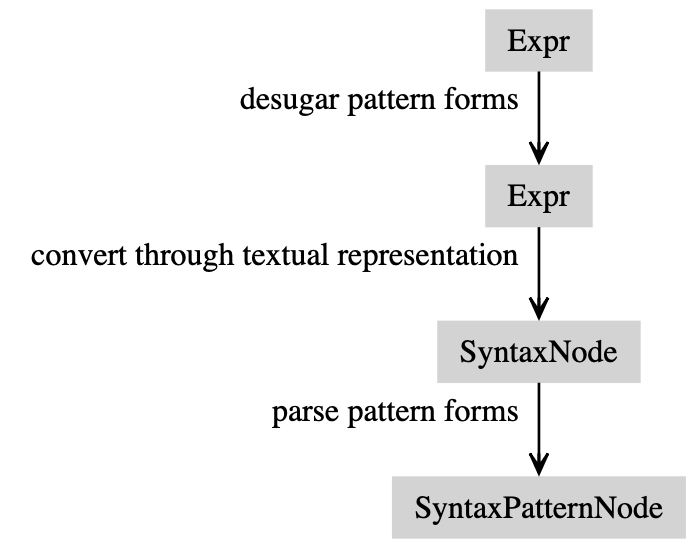
\includegraphics[height=0.3\textwidth]{parser.png}
\end{figure}

The flaw is introduced in the \texttt{Expr} \(\to\) \texttt{SyntaxNode} step. Converting
an \texttt{Expr} to a \texttt{SyntaxNode} based on textual representation is not
always reliable. Though few in number, certain differences exist
between the two representations \cite{expr_vs_syntaxnode}. A notable
disparity concerns implicit \texttt{block} nodes. \texttt{Expr} includes extra
\texttt{block}s in order to attach \texttt{LineNumberNodes} to its children. This is
the case for a short form function definition:

\begin{lstlisting}[language=julia]
julia> :( f(x) = 2 )
:(f(x) = begin
          #= REPL[16]:1 =#
          2
      end)
\end{lstlisting}

\texttt{SyntaxNode}s inherently store source location information and hence
don't require extra nodes:

\begin{lstlisting}[language=julia]
julia> parsestmt(SyntaxNode, "f(x) = 2")
SyntaxNode:
[function-=]
  [call]
    f                                :: Identifier
    x                                :: Identifier
  2                                  :: Integer
\end{lstlisting}

Argus uses the \texttt{Expr} representation for parsing and the \texttt{SyntaxNode}
one for matching. This causes unexpected behaviour when the
representations differ:

\begin{lstlisting}[language=julia]
julia> syntax_match((@pattern f(x) = 2), parsestmt(SyntaxNode, "f(x) = 2"))
MatchFail("no match")

julia> syntax_match((@pattern f(x) = 2), parsestmt(SyntaxNode, "f(x) = begin 2 end"))
BindingSet with 0 entries
\end{lstlisting}

A robust translation from \texttt{Expr} to \texttt{SyntaxNode} would solve this
problem.

The syntax matching mechanism could be extended to support
templates. This would allow Argus to serve as a tool for writing
macros, aligning it more closely with \texttt{syntax/parse}. The rule
framework could then be improved as well by adding suggestions and
code refactoring.

Another limitation comes from Argus's pattern fail conditions. A
satisfied fail condition causes a match failure. It is not possible to
report a source node that fits the superficial layout of a pattern,
but does not meet certain criteria. The value of \emph{late failures} is
demonstrated by the \texttt{let} example from section \ref{sec:org0a134f1}:

\begin{lstlisting}[language=racket]
(define-syntax (let stx)
  (syntax-parse stx
    [(let ([var:identifier rhs:expr] ...) body:expr)
     #:fail-when (check-duplicate #'(var ...))
                 "duplicate variable name"
     #'((lambda (var ...) body) rhs ...)]))
\end{lstlisting}

\texttt{(let ([a 1] [b 2]) (+ a b))}

\hspace{0.3cm}\textit{compile-time expansion}: \texttt{((lambda (a b) (+ a b)) 1 2)}

\hspace{0.3cm}\textit{run-time result}: \texttt{3}

\vspace{0.25cm}

\texttt{(let (["a" 1]) (add1 a))}

\hspace{0.3cm}\textit{compile-time error}: \texttt{expected identifier}

\vspace{0.25cm}

\texttt{(let ([a 1] [a 2]) (+ a a))}

\hspace{0.3cm}\textit{compile-time error}: \texttt{duplicate variable name}

\vspace{1em}

The goal is for a \texttt{let} definition to match the pattern \texttt{(let
([var:identifier} \texttt{rhs:expr] ...) body:expr)} and \emph{report an error} if
there are duplicate bindings. Argus would simply return no match in
case of misuse of a structurally matching source node, just as it
would for a structurally unrelated source node. Late failures are
especially relevant for writing macros.

\texttt{syntax/parse} sets a noteworthy precedent in reporting errors
\cite{fortifying_macros}. Argus could follow the example and learn to
provide more specific failure messages.

User-oriented improvements include compiling a default set of static
analysis rules and offering a command line interface. The latter
depends on current possibilities for ahead-of-time compilation in
Julia \cite{julia_aot}.

\section{Conclusions}
\label{sec:org757539b}

We have shown that Julia can learn from languages with advanced
metaprogramming support in order to provide powerful tools for
examining and manipulating syntax. We introduced Argus.jl as a more
expressive alternative to other existing Julia static analysis
packages. Its core concepts and driving algorithms have been discussed
at length. All underlying mechanisms have been illustrated through
step-by-step examples.

We have proven Argus's practical applicability in a real-world use
case. Its flexibility was demonstrated by its ability to successfully
match source code while gathering and logging information in a
specified format.

In the future, Argus could be more tightly integrated with Julia's
metaprogramming system. It could continue to draw inspiration from
other programming languages in order to select and report specific
errors in case of misuse. Its rule writing engine could be presented
as a command line tool that scans files and refactors code. Argus
could expose a set of default static analysis rules readily available
for use.

\section{Acknowledgements}

I am grateful to JuliaHub for providing me with the necessary context
for carrying out this endeavour.
I would also like to thank my partner, Andrei, for the invaluable
support he gave me throughout the entire process. His technical
advice and aesthetic recommendations not only improved the quality
of this work, but also strengthened my software design skills.
My gratitude goes to my coordinating professor as well, whose
courses have inspired me to pursue the challenging yet rewarding field
of compilers.
Last but not least, I want to thank my colleagues and friends who have
read iterations of this paper in great detail and pointed out the
mistakes and ambiguities they encountered.

\input{bib.tex}

\end{document}

% Inspired by the International Journal of Computer Applications template
